\begin{equation}
    \begin{aligned}
        &\quad \int \ee^{\ii q_1 \cdot x} \dd{x} \int \ee^{\ii q_2 \cdot y} \dd{y} \int \ee^{- \ii p \cdot z} \dd{z} 
    \begin{gathered}
        \begin{tikzpicture}[x=0.75pt,y=0.75pt,yscale=-1,xscale=1]
            %uncomment if require: \path (0,300); %set diagram left start at 0, and has height of 300
            
            %Shape: Circle [id:dp7977208390713126] 
            \draw   (224,171.35) .. controls (224,156.25) and (236.25,144) .. (251.35,144) .. controls (266.46,144) and (278.71,156.25) .. (278.71,171.35) .. controls (278.71,186.46) and (266.46,198.71) .. (251.35,198.71) .. controls (236.25,198.71) and (224,186.46) .. (224,171.35) -- cycle ;
            %Straight Lines [id:da24233957833824893] 
            \draw    (169.29,171.35) -- (224,171.35) ;
            %Straight Lines [id:da32762511162194086] 
            \draw    (269.29,151.35) -- (300.71,107.56) ;
            %Straight Lines [id:da9552561758852673] 
            \draw    (267.29,194.56) -- (307.71,246.53) ;
            
            % Text Node
            \draw (167.29,171.35) node [anchor=east] [inner sep=0.75pt]    {$z$};
            % Text Node
            \draw (302.71,104.16) node [anchor=south west] [inner sep=0.75pt]    {$x$};
            % Text Node
            \draw (309.71,249.93) node [anchor=north west][inner sep=0.75pt]    {$y$};
            \end{tikzpicture}            
    \end{gathered} \\
    &= \frac{\ii}{q_1^2 - m^2 + \ii 0^+} \frac{\ii}{q_2^2 - m^2 + \ii 0^+} \frac{\ii}{p^2 - m^2 + \ii 0^+} (2\pi)^4 \delta^{(4)}(q_1 + q_2 - p)
    \begin{gathered}
        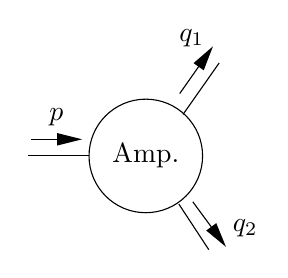
\begin{tikzpicture}[x=0.75pt,y=0.75pt,yscale=-1,xscale=1]
            %uncomment if require: \path (0,300); %set diagram left start at 0, and has height of 300
            
            %Shape: Circle [id:dp7977208390713126] 
            \draw   (224,171.35) .. controls (224,156.25) and (236.25,144) .. (251.35,144) .. controls (266.46,144) and (278.71,156.25) .. (278.71,171.35) .. controls (278.71,186.46) and (266.46,198.71) .. (251.35,198.71) .. controls (236.25,198.71) and (224,186.46) .. (224,171.35) -- cycle ;
            %Straight Lines [id:da24233957833824893] 
            \draw    (194.71,171.35) -- (224,171.35) ;
            %Straight Lines [id:da32762511162194086] 
            \draw    (269.29,151.35) -- (286.71,126.56) ;
            %Straight Lines [id:da9552561758852673] 
            \draw    (267.29,194.56) -- (281.71,216.53) ;
            %Straight Lines [id:da02229538950783616] 
            \draw    (195.94,163.35) -- (218.65,163.35) ;
            \draw [shift={(220.65,163.35)}, rotate = 180] [fill={rgb, 255:red, 0; green, 0; blue, 0 }  ][line width=0.08]  [draw opacity=0] (12,-3) -- (0,0) -- (12,3) -- cycle    ;
            %Straight Lines [id:da8847128858390558] 
            \draw    (267.71,141.28) -- (282.55,120.19) ;
            \draw [shift={(283.71,118.56)}, rotate = 485.15] [fill={rgb, 255:red, 0; green, 0; blue, 0 }  ][line width=0.08]  [draw opacity=0] (12,-3) -- (0,0) -- (12,3) -- cycle    ;
            %Straight Lines [id:da23645625787636826] 
            \draw    (274,193.46) -- (288.81,213.57) ;
            \draw [shift={(290,215.18)}, rotate = 233.63] [fill={rgb, 255:red, 0; green, 0; blue, 0 }  ][line width=0.08]  [draw opacity=0] (12,-3) -- (0,0) -- (12,3) -- cycle    ;
            
            % Text Node
            \draw (251.35,171.35) node   [align=left] {Amp.};
            % Text Node
            \draw (208.29,157.95) node [anchor=south] [inner sep=0.75pt]    {$p$};
            % Text Node
            \draw (280.71,120.16) node [anchor=south east] [inner sep=0.75pt]    {$q_{1}$};
            % Text Node
            \draw (292,211.78) node [anchor=south west] [inner sep=0.75pt]    {$q_{2}$};
            \end{tikzpicture}                     
    \end{gathered} \\
    &= \frac{\ii}{q_1^2 - m^2 + \ii 0^+} \frac{\ii}{q_2^2 - m^2 + \ii 0^+} \frac{\ii}{p^2 - m^2 + \ii 0^+} \mel{q_1, q_2}{S}{p} .
    \end{aligned}
\end{equation}